% Removed from manuscript at author request; immutable raw results remain in their original packages.
\subsection{Local-document continuation microbenchmark}
\label{sec:e1-timing}
The timing experiment compares three instrumented configurations of the pinned Qwen3.6-27B-FP8 stack on GB10: native MTP with five drafts, native MTP with eleven drafts, and the selected cat10 tree route. Cat10 has ten nodes including the root, maximum draft-path depth five, and padding to sixteen nodes. Native MTP-5 is depth-comparable; MTP-11 is a longer-chain control. Both native arms use stock MTP paths within the same patched runner as the tree, with tree decoding disabled and no tree descriptor. Their attention backend is \texttt{FLASH\_ATTN}; the tree uses \texttt{TREE\_ATTN}. Thus these are comparisons of implemented configurations, not isolated changes to the GDN arithmetic.

The frozen design has eighteen cells: three arms, actual batch sizes one and four, and three paired blocks, with a fresh server boot for each cell and a fixed order that rotates the arms across blocks. All arms use eager execution, synchronous scheduling, disabled prefix caching, temperature zero, and the same forward timer and output-event recorder. Heavy operand, hidden-state, and full-logit captures are disabled. The workload is a local-document continuation microbenchmark: eight frozen excerpts from this repository's internal design and experiment documents, four of 256 tokens and four of 4096 tokens. They were selected from the 96-prefix pool by context length and the native model's top-two logit margin, two per stratum, and reused from E7a. Each excerpt is sent to the raw completions endpoint with a 128-token output budget and EOS enabled. These are text-continuation requests, not SWE-bench Verified issues: there is no coding-agent tool loop, patch generation contract, or task evaluator. B1 submits them sequentially; B4 submits two fixed cohorts of four. Matching input prefixes does not establish identical generated continuations. Warm-up consists of two 32-token requests using the first prefix at B1, or one 32-token-per-request cohort using the first four prefixes at B4. This does not guarantee that every later shape is warm; valid slow intervals remain in the measurement. An untimed preflight within the first boot of each native arm/batch condition passed before warm-up and timing; a final sealed-ledger audit also passed. Later boots reuse that qualification. These preflights are finite route checks, not full-model equivalence tests.

For each cell the primary rate is
\begin{equation}
 R = \frac{\sum_{j\in\mathcal{I}} n_j}
 {\sum_{j\in\mathcal{I}}(t_{j+1}-t_j)},
\end{equation}
where $n_j$ counts returned API token IDs assigned to physical step $j$, and $t_j$ is its recorded start timestamp at the wall-mark hook. The set $\mathcal{I}$ is restricted to the timed phase: adjacent physical-step and full-forward indices must describe pure decode with the same active request set and declared occupancy, without an intervening mixed/prefill forward or chain break. Preflight and warm-up intervals are excluded, while their outputs remain in token reconciliation. Each physical interval appears once in the denominator, including at B4. The first pure step is retained when it has an eligible successor; terminal steps without a successor, mixed/prefill steps, phase breaks, and changes in cohort or occupancy are excluded. Their outputs remain in the token reconciliation. All eligible slow intervals are retained; a 1.5-second cutoff supplies a diagnostic only. Recorder loss or missing API evidence invalidates the whole cell. Each B1 prompt and each B4 cohort must supply at least one eligible interval; these are coverage floors, not precision guarantees. The metric is retained-decode output rate, not full-service latency. Any component subtraction must use the same event support, and its residual is not identified as host time.

The analysis reports cell rates and the mean of three boot rates per arm, separately for B1 and B4. B4 is aggregate output throughput across four active requests; neither column reports a selected best boot. For tree minus MTP-5, tree minus MTP-11, and MTP-11 minus MTP-5, it resamples the three whole paired blocks 10,000 times with fixed seed 20260921 and reports a 95\% percentile interval for the mean paired rate difference. The prespecified practical precision target is interval half-width at most 10\% of the mean MTP-5 rate. Three blocks provide coarse uncertainty; no independently measured between-boot pilot variance justified that replication count. Only sealed VALID cells contribute rates. An arm mean requires all three blocks; a contrast is not estimable without all three paired blocks and a complete native-MTP-5 normalization baseline. The initial eighteen cells remain the primary reporting set, including insufficient-support and invalid outcomes without imputation or unpaired replacement, and all precision misses. No prompt replacement, output-budget extension, or favorable repetition is permitted.

\paragraph{Engine-seed deviation}
The frozen settings specified seed 20260921. All API requests use that seed, and both native engines use it, but the tree launcher omits the engine-seed option and uses the logged default zero. Review identified this deviation during the first tree boot; the original plan, snapshots, and campaign are preserved, with a dated addendum. The loaded greedy duplicate-source selector uses a separate explicit generator; inspection found no global-engine-seed input at that selector. This source observation does not prove whole-engine seed invariance or exclude effects elsewhere. The comparison therefore describes the configurations as executed and cannot identify a seed-controlled causal effect of the tree algorithm. Paired uncertainty intervals do not remove this configuration difference, and a passing measurement seal does not mean complete compliance with every frozen setting.

\paragraph{Measured outcomes}
All eighteen initial cells completed with valid sealed token/event evidence; no cell was replaced or extended. B1 cells retained 249--314 physical intervals each, with at least 24 per prompt. B4 cells retained 51--64 full-cohort intervals each, with at least 25 per cohort. No eligible interval exceeded the 1.5-second diagnostic cutoff. All-phase API reconciliation includes the preflight and warm-up outputs, while the primary numerator and denominator use timed support only. Cell 16's p021 response ended at EOS after 101 tokens; every other timed response used the 128-token budget. Its eight-prompt coverage remained valid, so this outcome is retained. The artifact reports every cell, per-prompt/cohort support, termination, and exclusions; terminal intervals without a successor have unobserved duration rather than an imputed zero.

Figure~\ref{fig:e1-timing} reports the complete initial campaign. On this local-document workload, mean retained-decode rates for native MTP-5, native MTP-11, and cat10 are respectively 13.67, 11.44, and 12.69 tokens/s at B1, and 55.38, 42.15, and 47.28 tokens/s at B4. Cat10 is 7.14\% below MTP-5 at B1 and 14.61\% below it at B4, while exceeding the longer-chain MTP-11 configuration. The paired cat10-minus-MTP-5 differences are $-0.976$ tokens/s at B1 (95\% percentile interval $[-1.085,-0.787]$) and $-8.091$ at B4 ($[-9.680,-5.830]$). Against MTP-11 they are $1.256$ ($[1.157,1.445]$) and $5.133$ ($[4.179,6.811]$). All six contrasts, including MTP-11 minus MTP-5, meet the prespecified precision target; the largest half-width divided by the mean MTP-5 rate is 4.82\%. This does not turn the coarse three-block intervals into evidence of broad workload precision.

\begin{figure*}[t]
\centering
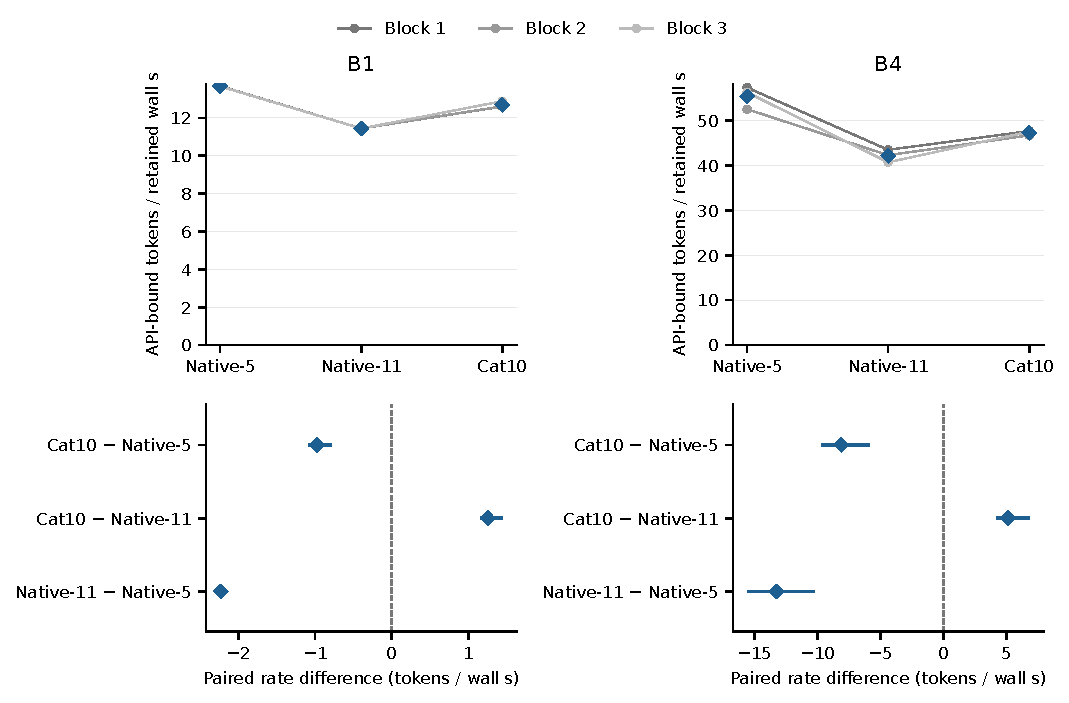
\includegraphics[width=0.94\textwidth]{figures/e1-timing.pdf}
\caption{E1, local-document continuation: all eighteen initial fresh-boot cells on eight internal-document excerpts, with 256/4096-token contexts and a 128-token output limit. Top: each gray line connects one paired block; blue diamonds mark the mean of three boot rates. Bottom: mean paired differences and the frozen 95\% bootstrap percentile intervals, resampling whole blocks separately at B1 and B4. Rates bind returned API tokens to unique retained wall intervals. These are as-executed instrumented configurations with different attention backends, the disclosed engine-seed deviation, and observed output divergence; they do not isolate a causal tree-algorithm effect.}
\label{fig:e1-timing}
\end{figure*}

\paragraph{Observed continuation divergence}
A retrospective comparison uses the complete timed API-ID streams, not just rate-support tokens. Across the three pairs of arms, three blocks, two batch conditions, and eight prompts, only 14 of 144 same-block prompt-stream pairs are exactly equal. Comparing the three block pairs within each arm/batch gives 72 equal pairs out of 144. Both native B1 arms repeat exactly in all 24 within-arm comparisons apiece; tree B1 does so in 8/24. At B4 the equality counts are 7/24 for MTP-5, 5/24 for MTP-11, and 4/24 for cat10. These dependent pair counts describe the observed streams, not an estimated population failure probability. They neither identify the source of divergence nor establish full-model sequential equivalence. Together with the seed and backend differences, they limit the result to measured output rates of the tested configurations on fixed input prefixes. No matched-continuation, quality-preservation, or isolated algorithm-speedup claim follows. The retrospective diagnostic does not alter the frozen eligibility, rates, intervals, or precision decisions.

\subsection{Single-logits reuse: qualified component comparison}
\label{sec:e8-timing}
E8 uses the same eight-prefix local-document continuation workload as E1 and isolates the redundant vocabulary projection described in Section~\ref{sec:optimization}. The E1 tree already uses logits reuse. E8 adds a real source-controlled OFF path that recomputes the head for spine selection while retaining the same first-logits candidate extraction. The actual loaded source, rather than an inert environment switch, defines each arm. Cat10 topology, stock \texttt{TREE\_ATTN}, flat-slot KV remapping, model weights, image, B1 occupancy, eager execution, synchronous scheduling, disabled prefix caching, and temperature zero remain fixed. Both engine and API seeds are explicitly 20260921.

Two untimed qualification boots preceded timing. On each of eight frozen prefixes, each arm returned 32 API token IDs. Every qualified proposal evaluated both head paths on the same input: 103 proposals and 515 paired head comparisons per arm passed bitwise whole-logit, argmax, ordered top-two, and packed candidate-tree checks. The gate also checked input/RNG preservation and watched-tensor mutation, with closed recorder and head receipts. Complete API streams reconciled with the emitted ledger, and all eight streams matched across these two qualification boots. These finite checks establish the observed head/candidate invariants; they are not a full-model state-equivalence proof and supply no timing estimate.

The timing campaign then ran three fixed paired blocks in OFF/ON, ON/OFF, and OFF/ON order. Each of the six fresh servers received two 32-token warmups followed by the same eight prefixes at a 128-token budget with EOS enabled. Expensive paired-head checks and captures were disabled; small head-call counters remained in both arms. The final census confirms five vocabulary projections per proposal with reuse ON and ten with reuse OFF. All ten requests in each boot are included in API/ledger reconciliation. The primary rate uses the same retained-decode token/wall support as E1, with at least one eligible interval per timed prefix, all valid slow intervals retained, and no failed-cell replacement or prompt selection. GPU ownership was sampled before, every five seconds during, and after the workload. Every observed GPU process belonged to the single owned container; this does not exclude transient contention between samples.

The prespecified primary statistic is the mean of three paired relative rate differences,
\begin{equation}
 \Delta_{\mathrm{reuse}}=\frac{1}{3}\sum_{b=1}^{3}
 \left(\frac{r_{b,\mathrm{ON}}}{r_{b,\mathrm{OFF}}}-1\right).
\end{equation}
The frozen analysis resamples whole paired blocks 10,000 times with seed 20260921 and reports the 2.5th and 97.5th percentiles. All three complete pairs are required; uncertainty from three blocks is coarse. The ratio of arm means is a secondary diagnostic. The estimator was fixed before any timing data.

\begin{table}[t]
\caption{E8, local-document continuation: all three paired B1 blocks on the same eight excerpts as E1. Rates are retained-decode tokens/s for the source-controlled head-reuse comparison. The final ON boot has different continuations and one early EOS; it remains in the primary analysis.}
\label{tab:e8-reuse}
\centering\footnotesize
% Generated only from the complete independently reviewable frozen E8 aggregate.
\begin{tabular}{@{}lrrr@{}}
\toprule
Block & Reuse OFF & Reuse ON & Paired change \\
\midrule
1 & 9.686 & 12.591 & +29.99\% \\
2 & 9.703 & 12.595 & +29.81\% \\
3 & 9.697 & 12.887 & +32.90\% \\
\bottomrule
\end{tabular}

\end{table}

All six initial cells completed with valid sealed evidence. They retained 298--314 intervals each, with at least 29 per prefix and no eligible interval above the 1.5-second diagnostic cutoff. Mean boot rates are 12.691 tokens/s with reuse ON and 9.695 with reuse OFF. The mean paired relative increase is 30.90\%, with a frozen 95\% percentile interval of $[29.81\%,32.90\%]$. Table~\ref{tab:e8-reuse} reports every pair; no run was repeated or replaced. E1 already includes this optimization, so its Cat10 rate must not be multiplied by this relative increase.

Complete timed streams match in 16 of 24 within-pair comparisons and 32 of 48 across-block comparisons within an arm. The third ON boot differs on all eight prefixes; p021 ends at EOS after 101 tokens. Its support remains valid and its outcome is retained. Thus the component contrast reports rates of these as-executed instrumented configurations on fixed prefixes, not equal-output latency or general quality preservation. Same-input head equivalence, reduced head-call count, and cross-boot continuation equality are separate claims. E8 adds B1 attribution evidence for this component; it neither replaces the E1 native/tree comparison nor establishes a fully optimized or composed system gain.

